%
% you should only have one "documentclass" line.  the following lines
% are samples that give various options.  the nofrontmatter option is
% nice because it suppresses the title and signature pages when you want
% to focus only on the main body of the thesis
%
% Friday April 10 2010 Ray Hylock <ray-hylock@uiowa.edu>
% documentclass options:
%   abstractpage            if you want to add an internal abstract (optional)
%   ackpage                 if you would like to add an acknowledgements page (optional)
%   algorithms              if you want a list of algorithms (optional)
%   appendix                if you have an appendix (optional)
%   copyrightpage           if you wish to copyright your thesis (optional)
%   dedicationpage          if you wish to make a dedication (optional)
%   epigraphpage            if you would like to add an epigraph to the beginning of your thesis (optional)
%   examples                if you want a list of examples (this uses the ntheorem package)
%   exampleslemmas          if you want a combined list of examples and lemmas (this uses the ntheorem package) (optional)
%   examplestheorems        if you want a combined list of examples and theorems (this uses the ntheorem package) (optional)
%   exampleslemmastheorems  if you want a combined list of examples, lemmas, and theorems (this uses the ntheorem package) (optional)
%   figures                 if you have any figures (this is required if you have even one figure)
%   lemmas                  if you want a list of lemmas (this uses the ntheorem package) (optional)
%   lemmastheorems          if you want a combined list of lemmas and theorems (this uses the ntheorem package) (optional)
%   nofrontmatter           suppresses the title and signiture pages for working on the body
%   tables                  if you have any tables (this is required if you have even one table)
%   theorems                if you want a list of theorems (this uses the ntheorem package) (optional)
%   phd                     if phd student; this will add the doctoral abstract (mandatory for PhD and DMA thesis candidates only)
%

% full options
%\documentclass[phd,abstractpage,copyrightpage,dedicationpage,epigraphpage,ackpage,figures,tables,lemmas,appendix]{uithesis}

% common options
%\documentclass[phd,dedicationpage,ackpage,figures,tables,appendix]{uithesis}

% example
\documentclass[phd,appendix,figures]{uithesis}

%=============================================================================
% User packages
%=============================================================================
\usepackage{bookmark}	% [recommended] for PDF bookmark generation
\usepackage{blindtext} 	% example text generation
\usepackage[ruled,chapter]{algorithm}  % display algorithms
\usepackage[super,comma,sort,numbers]{natbib}
% to place figures/subfigures
\usepackage{graphicx}
\usepackage{subfig}
% path to figures
\graphicspath{{img/Aim1/}{img/Aim2/}{img/Aim3/}{img/CurrentStudy/}{img/GeneralDiscussion/}{img/GeneralMethods/}{img/Introduction/}}
\usepackage{forloop} % for loops display images
\usepackage{hyperref} % to insert hyperlinks
\usepackage{textcomp} % to write degree symbols
\usepackage{float} % image placement
% for smaller captions
\usepackage[labelfont=bf]{caption}
\captionsetup{font=footnotesize}
% https://tex.stackexchange.com/questions/370278/is-there-any-reason-to-use-inputenc
\usepackage[utf8]{inputenc} % for non-ascii characters
\newcommand{\comment}[1]{}
%=============================================================================
% prelude
%=============================================================================

\title{Task Related Correlations}
\author{James Kent}
\dept{Neuroscience}

% multipleSupervisors=true for two advisors
\setboolean{multipleSupervisors}{false}
\advisor{Assistant Professor Dr. Michelle Voss}
% for multiple advisors; change <value> to line up the names
%\setboolean{multipleSupervisors}{true}
%\advisor{Advisor 1\\\hspace{<value>mm}Advisor 2...}
%
% edit the names below to have your committee members names appear
% on the signature page.  memberOne should be your advisor.
%
\memberOne{Michelle Voss}
\memberTwo{Eliot Hazeltine}
\memberThree{Vincent Magnotta}
\memberFour{Jatin Vaidya}
\memberFive{Jan Wessel}
\submitdate{May 2020}
\copyrightyear{2020}

\Abstract{
\blindtext
}

%\dedication{Dedication here (optional)}

%\epigraph{Epigraph here (optional)}

%\acknowledgements{Acknowledgements here (optional)}

\begin{document}

\frontmatter

%=============================================================================
\chapter{Introduction}
%=============================================================================

What makes us human?
What makes us "different" than robotic automatons that blindly react to their environment?
Some may say free will, but perhaps they are really thinking of cognitive control.
Cognitive control is the ability to take into account context to decide what action to take in response to a stimulus. 
A common example is driving.
If you are driving through a neighborhood with notoriously short yellow lights, I would hope you are likely to stop when you see a light turn yellow.
On the other hand, if you are driving through a neighborhood where the yellow light lasts for eight, maybe ten seconds, you may cruise through the intersection.
The two automaton behaviors are the braking and continuing (maybe speeding up a little) through the yellow light.
Cognitive control represents the process that selects one of the two behaviors.
In this example, cognitive control is informed by the spatial location of the driver and the location's association with either a short or long yellow light.

There is a vast sea of cognitive control research: its ontology, its neural basis, when it breaks down, but several key gaps still remain ~\citep{Gratton2017,Dosenbach2010,Braver2000}.
\textbf{The first key gap is how neural networks are represented during a task that requires cognitive control}.
The current literature has found which brain regions are associated with cognitive control and what networks those regions participate in at rest ~\citep{Gratton2017a,Lerman-Sinkoff2017,Herd2006,Rizio2012,Cooper2015,AppelBaum2014,Dosenbach2007}.
However, the crucial missing evidence is directly observing the networks during a task.
The reason this evidence does not exist is because of the lack of available methods.
By creating and sharing this method, we will provide more direct evidence for cognitive control networks.

\textbf{The second key gap is how cognitive control networks correlate with behavior}.
Related to the first gap, researchers have correlated brain activation and networks at rest with behavior, but not networks during a task. ~\citep{nomura2010b,Egner2004,Gonthier2016a,Braver2010,Huang2017}
The present research seeks to provide a more definitive connection between proposed cognitive control networks and behavior.

We've used driving as a behavior, but how is cognitive control measured in the lab?
In the lab, we don't use cars and pedals, we use pictures.
These pictures present conflicting information the viewer must disern given the context.
A classic task in this domain is Stroop.
In this task, the viewer must ignore the word (the automatic response) and report the color of the font (the controlled response).
The conflict arises when the word is a different color than its font color (e.g., the word red colored in blue font).
Thus, by looking at the reaction time difference between trials with  and without conflict, we can measure the cost to engage cognitive control in order to override an automatic response (however, there are alternative explanations) ~\citep{Hommel2011}. 
We can establish a relationship between network connectivity and reaction time cost with the above measures, and connect the construct of cognitive control with anatomy ~\citep{Braver2008,Dosenbach2007}.

\section{History of Cognitive Control}

To understand cognitive control, we must first take a step back to understand the theories that connected an individual's environment with their responses, presumably through the 3 pound piece of pulsating meat between our ears.
The 1960s were a tumultuous time of drugs, protests, and revolutions. 
Not to be outdone by the social and political environments, psychology staged its own revolution, a cognitive revolution against a backdrop of behaviorism, although the concept of revolution may be romanticizing what actually happened ~\citep{Leahey1992}. 
The gelatinous black box of the brain needed to be unveiled, and cognitive psychology was determined to pull back the curtain. 

One of the first cognitive models to gain traction during the "revolution" was Sternberg's serial processing model.
As the name suggests, Sternberg's serial processing model suggested people processed stimuli one at a time, serially, which gave psychology groundbreaking concepts such as the primacy and recency effects ~\citep{Sternberg1966}.

However, as with all models, serial processing was inadequate in explaining the flexibility of human cognition.
Namely, the deficit was the thought that human cognition was treated as an open loop system, where information was processed in stages and produced behavioral output. 
While closed-loop systems were pervasive in the subfield of cybernetics, the idea did not really pierce the veil of psychology until 1970 when Gregory published about the distinction between top-down and bottom-up processing ~\citep{Gregory1970}.
With the knowledge that people behave differently to the same stimulus depending on the context, psychologists concluded that in addition to feed-forward processing, there must also be a feedback mechanism to inform the appropriate response ~\citep{Gregory1970}.
The seed of cognitive control was planted.

Following this line of thought, Shriffrin \& Schneider differentiated the top-down and bottom-up processes, otherwise known as controlled and automatic processes by looking at processing speed, attentional load, and capacity ~\citep{Shiffrin1977}. 
They derived three fundemental attributes of cognitive control.
One, controlled processes are slower relative to automatic processes. 
Two, controlled processes are in competition with automatic processes. 
And three, controlled processes tap into a shared limited resource.

The next major model of cognition that involved feedback (controlled processing) was Norman and Shallice's (1986) supervisory attentional system (SAS) ~\citep{Norman1986}. 
The SAS encompasses slow, deliberate top-down processes when pursuing the habitual response is incorrect or inadequate.
Around the same time Baddeley released a model of working memory which included a Central Executive where putative functions of cognitive control would be performed ~\citep{Baddeley1996}.
However, as Baddeley noted himself, his concept of the central executive was too vague and could only "serve as little more than a ragbag" (p.6). 
Researchers have found this ambiguous cloud of higher cognition within the central executive, but efforts to divide it up into useful chunks has evaded strong empirical scrutiny for years.

Miyake et al. (2000) tackles the central executive head on and began carving the construct into distinct components. 
Their group found that executive function could be split into three categories:
1) shifting between tasks or mental sets,
2) updating and monitoring of working memory representations, and
3) inhibition of dominant or prepotent responses ~\citep{Miyake2000}.
This work was instrumental towards providing a stronger behavioral definition of cognitive control, and paved the way for well designed imaging studies to study cognitive control.
Miyake provided an excellent first-pass into dividing up the central executive, but more detailed explanations are needed.
For example, the congruency sequence effect (i.e. Gratton effect) would require monitoring of working memory representations and inhibition of a dominant response in favor of a less dominant response, but do these processes occur over the course of the task between stimulus presentations, or perhaps they are engaged when the stimulus is presented, or perhaps a mixture of both?

Braver added a much needed explicitness and computational validity to cognitive control. With his detailed, testable models, Braver began to peer into the conceptual void of the central executive and its anatomical underpinnings ~\citep{Braver2001}. 
He proposed a gating model, where phasic dopamine release in the prefrontal cortex (PFC) allowed for flexible updating of the active memories being held in place.

To illustrate, imagine a color stroop task where the participant has to name the color of the font, and ignore the word that is printed.
The foundation of the stroop task assumes that reading is an automatic process that requires little to no control, whereas naming the color is a controlled process that can act in opposition to reading if the printed word is also a color (e.g. the word blue colored in red font).
The maintenance of the goal (name the font color, not the word) is held in working memory (in the PFC), and the ability to acquire and maintain this goal is hypothesized to be a result of phasic dopamine release. 
If there was a long sequence of congruent trials (e.g. the word red with the font color red), the participant may take a shortcut and use the automatic process of naming the word.
An incongruent trial may appear after this sequence of congruent trials, and then the participant has to engage the controlled process through phasic dopamine release into the PFC.
Again, a common thread of these models does not lay with their accuracy to describe all of human cognition, but with their utility to frame our thoughts and describe particular aspects of human cognition. 

% add section for conflict monitoring theory (CMT)
\section{Conflict Monitoring Theory}
TODO
% add section for Prediction of Response-Outcome (PRO)
\section{Prediction of Response-Outcome}
TODO

\section{Dual Mechanisms of Control}

As mentioned in the previous section, an additional layer of nuance emerges when one asks exactly when is cognitive control engaged.
Is cognitive control engaged when the stimulus/probe appears or is it maintained over the course of the task?
Does it matter?
Is it all a part of the same process?
Braver has classified the above circumstances as different forms of cognitive control, reactive and proactive, and they form the Dual Mechanisms of Control (DMC) framework ~\citep{Braver2012}.
A way to conceptualize proactive and reactive control is early selection and late correction, respectively ~\citep{Jacoby1999}.
Early selection means the goal is held in working memory either for the duration of the task, and/or the period between a cue and a probe.
Late correction, on the other hand, means the goal is not held in working memory, rather, the decision about whether the automatic or the controlled behavior set should drive behavior is not engaged until a probe or stimulus is seen.
Braver found this behavioral distinction between proactive and reactive cognitive control while working on the AX version of the continuous performance task (AX-CPT) ~\citep{Paxton2008}.
The AX-CPT is a task where participants are to respond to a particular cue-probe pair, namely A-X.
All other cue-probe pairs (A-Y, B-X, B-Y) should be ignored and the participant should not respond to the probe on those trials.
This task becomes difficult because the A-X trials occur with a high probability (e.g. 70\%) developing an expectancy to respond to this cue-probe pair.
Following this built up expectancy, two other cue-pairs become interesting, A-Y and B-X.
Participants may have built up an expectancy to respond to a probe after the target cue A, and/or built up an expectancy to respond to probe X even if it was preceded by a B cue.
The B-Y trials act as a control because there is no bias present in the cue or the probe to tempt the participant to respond incorrectly.
This task lends itself towards clear predictions of performance depending an individual is particularly engaging proactive or reactive cognitive control.
Specifically, if a participant was using a more proactive strategy or in other words, were using strong goal maintenance, we would expect to see improved B-X performance, but a diminished A-Y performance.
On the other hand, participants with impaired goal maintenance would be expected to perform reactively, showing poorer performance on the B-X trials relative to the A-Y trials ~\citep{Paxton2008}.

What populations may have poor goal maintenance?
One widely studied population, by Braver and others is healthy older adults.
Through Braver's proposed mechanism of less reliable dopamine signaling and poorer frontal lobe performance, the consequence of impaired goal maintenance is an increased reliance on reactive cognitive control, even in circumstances where proactive control would lead to better performance.
While this description of proactive and reactive cognitive control may lead one to believe that they are two ends on the same spectrum, the proposed separate neural architecture and recent behavioral evidence suggest they are semi-independent processes ~\citep{Gonthier2016}.
The difficulty in demonstrating their independence lays within producing a double dissociation.
Schizophrenia and aging provide excellent models of proactive control breaking down, but there is not currently a model for the break down of reactive control in behavior that preserves proactive cognitive control.
Thus while one could theoretically use both proactive and reactive cognitive control, in practice the evidence suggests the engagement of proactive control results in a lesser need to engage reactive control ~\citep{Gonthier2016a}.
Taking the perspective that control is costly in terms of effort and neural resources, using both reactive and proactive control mechanisms strongly is wasteful.

\section{Neural Basis of Cognitive Control}

Akin to Ralphie's excitement when he got his Red Ryder air rifle, the world of neuroscience was abuzz with the advent of fMRI in 1990 ~\citep{Ogawa1990}. 
The ability to observe the inner machinations of the mind without costly surgeries and reliance on clinical populations greatly expanded the granularity of inquiry researchers were eager to ask. 
This was a boon for cognitive control as well because of the theoretical ambiguities outlined in the previous sections about the central executive.
Where is the center of control, could one point it out in a brain scan, or was it perhaps more complicated?
Cognitive Control saw its first debut in fMRI in 1995 with D'Esposito's search for the Central Executive ~\citep{DEsposito1995}. 
While Cognitive Control was not in the lexicon at the time of publishing, the markers for its existence were there in the prefrontal cortex.

Parallel to Braver's work, Dosenbach released a theoretical framework of cognitive control named dual mechanisms of cognitive control ~\citep{Dosenbach2007}. 
This model contained a quick/adaptive component and a longer sustained component.
Sound familiar?
Braver's conception of proactive and reactive cognitive control maps onto the slow sustained component and the quick/adaptive component, respectively ~\citep{Braver2012}.
The proactive component is anchored by the dorsal anterior cingulate cortex and anterior insula in the cingulo-opercular network ~\citep{Dosenbach2008}.
The reactive component is anchored by the lateral prefrontal cortex and the parietal cortex in the fronto-parietal network ~\citep{Dosenbach2008}.
A double dissociation between the fronto-parietal and cingulo-opercular networks has been demonstrated in a lesion study, providing further evidence of the network separability ~\citep{nomura2010b}.
While Braver has mentioned Dosenbach's analytical methods, serious inquiry mapping the relationship between proactive and reactive control with the fronto-parietal and congulo-opercular networks has yet to be established ~\citep{Braver2006,Cooper2015}.

\section{Intrinsic and Extrinsic Networks}

In the past decade and currently, accumulating evidence suggests intrinsic activity (i.e. what goes on in your brain when you aren't performing a task) is more than physiological noise and contributes meaningfully to behavior ~\citep{Busch2010,Kenet2003,McCormick1999,Mateo2017}.
This field of "resting state" imaging has established itself as a measure in the fMRI world that is likely not going away any time soon ~\citep{VandenHeuvel2010,Shen2015}.
Resting state imaging measures the spontaneous blood flow that occurs in the brain in the absence of a task.
Blood flow in some regions tend to co-occur with blood flow in spatially disparate regions, creating "functional" connectivity as measured through Pearson's Correlations or other connectivity measures.
Connectivity measures between regions (or between multiple regions known as networks) have been correlated with traits and behaviors with success ~\citep{Dennis2011,Duchek2013}.
Intervention studies have also seen changes in connectivity in relation to the behavior that was targeted ~\citep{Horowitz-Kraus2015}.
Some researchers attribute the functional connections between regions to Hebbian mechanisms, in which a simple interpretation is that "regions that fire together wire together" ~\citep{Harmelech2013}.
Thus if there is a long history of regions robustly communicating with each other, then we would be able to see that relationship represented in resting state.
However, there are many other sources that may contribute to resting state signal, such as motion, heartrate, non-neuronal processes, etc. ~\citep{Winder2017,Murphy2013}.

Given the multiple non-neurological sources of signals in resting state, another way to "boost" the signal of relevant networks is to observe them during a task ~\citep{Cole2014}.
In Cole (2014) they found increased connectivity in the fronto-parietal network from the task data, however in their model, they did not remove the impact of trial-to-trial variability, suggesting that the increased fronto-parietal connectivity could have been due to stimulus evoked connectivity and not due to a general state difference between rest and task.
The current study will use one regressor per trial to model residual connectivity, effectively removing the trial to trial variation the Cole (2014) modeling strategy left in.
Residual connectivity will measure the intrinsic connectivity and the additional task demands that are not directly related to the stimulus such maintaining goal information.
Thus residual connectivity represents both intrinsic and extrinsic network properties.

beta series, which measures the trial-to-trial variation of the brain's response to stimuli, mainly represents the extrinsic network, that is, connectivity induced by stimuli. ~\citep{Rissman2004}.
The trial-to-trial variance may also be influenced by intrinsic spontaneous fluctuations of the BOLD response that is ongoing throughout the task, and introduce correlations that are not directly related to seeing the stimulus ~\citep{He2013}.
However, as the Cole (2014) study found, the stronger fronto-parietal intra-network connectivity is likely due to the trial-to-trial variations of the BOLD response to stimuli.
The currently proposed study will interrogate this difference and provide a clearer contribution of stimulus evoked connectivity (beta series) and residual connectivity.


%=============================================================================
\chapter{Research Overview}
%=============================================================================

Advances in both fMRI analysis and theory of cognitive control have collided to produce ripe new areas to advance our understanding of cognitive control through fMRI ~\citep{Braver2012,Rissman2004,Mumford2012,Cisler2012}.
We can find evidence of cognitive control in our daily lives, from switching between an email and a conversation to making a quick decision behind the wheel. 
Specifically, cognitive control refers to the ability to use our context to inform our decisions. Cognitive control can be broken down into two modes, proactive and reactive ~\citep{Braver2012}. 
Proactive cognitive control encompasses the conflict preparation processes that occur for the entire duration of a task, and/or the conflict preparation between a cue and a stimulus.

In other words, the conflict processes that are not in direct response to a stimulus.
Reactive cognitive control, on the other hand, refers to the conflict adaptation that happens directly in response to a stimulus.
Two separable networks have been identified in proactive and reactive cognitive control, the cingulo-opercular (proactive) and fronto-parietal (reactive).
However, to this author's knowledge, there does not exist any research demonstrating the connectivity of these networks during a cognitive control task in fMRI.
Thus, the main thrust of this research is to establish these networks during a cognitive control task using two analytical methods theoretically sensitive to reactive or proactive cognitive control.

\begin{figure}[H]%
    \centering
    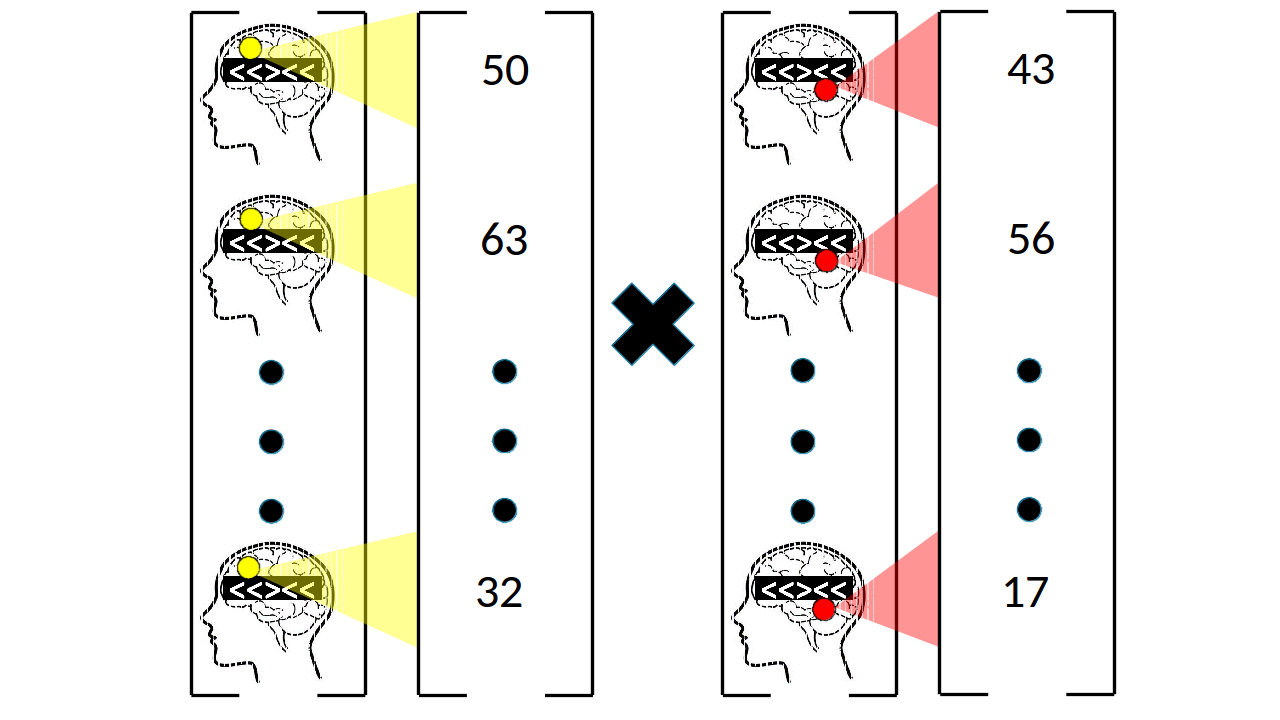
\includegraphics[scale=0.25]{betaseries_correlation_illustration}
    \caption{Setting up beta series Correlations. In the flanker task example above, betas (i.e. activation index) have been fit to every voxel per trial, and separated by condition (incongruent and congruent). This figure is only representing the incongruent trials, but both incongruent and congruent trial data can be collected.Regions of interest (ROIs) can be selected from these beta maps and all the voxels within the ROI are averaged. Once the betas are extracted from each ROI for each trial, the resulting lists of betas can be correlated with each other.}%
    \label{fig:betaseries_correlation_illustration}%    
\end{figure}

The first method is beta series correlations and is sensitive to the theoretical notion of reactive cognitive control (Figure ~\ref{fig:betaseries_correlation_illustration}). 
beta series correlations model the response after a congruent or incongruent stimulus capturing the "on-the-fly" conflict adaptations, otherwise known as reactive cognitive control.
Aim 1 will establish the use of this method due to its novel application to fast-event related designs of fMRI.

The second method is residual correlations; the time-course of the brain's activity after regressing out the stimulus onset information ~\citep{Fair2007,Cole2014,Bolt2017}. 
Residual correlations measure the theoretical notion of proactive cognitive control because proactive cognitive control represents the stable maintenance of goal-relevant task information throughout the performance of the task, which is what the time-series will represent.
Behavioral measures of proactive and reactive cognitive control exist, however outside of the AX-CPT it is difficult to analyze purely proactive and reactive behavioral components. 
Following the characterization of the purported reactive and proactive cognitive control networks, their relationship to existing behavioral measures will be established.
This research will contribute to the ongoing conversation of the neural basis of cognitive control, and provide a more direct metric of these networks during a  cognitive control task.

\section{Specific Aims}
\begin{figure}[H]%
	\centering
	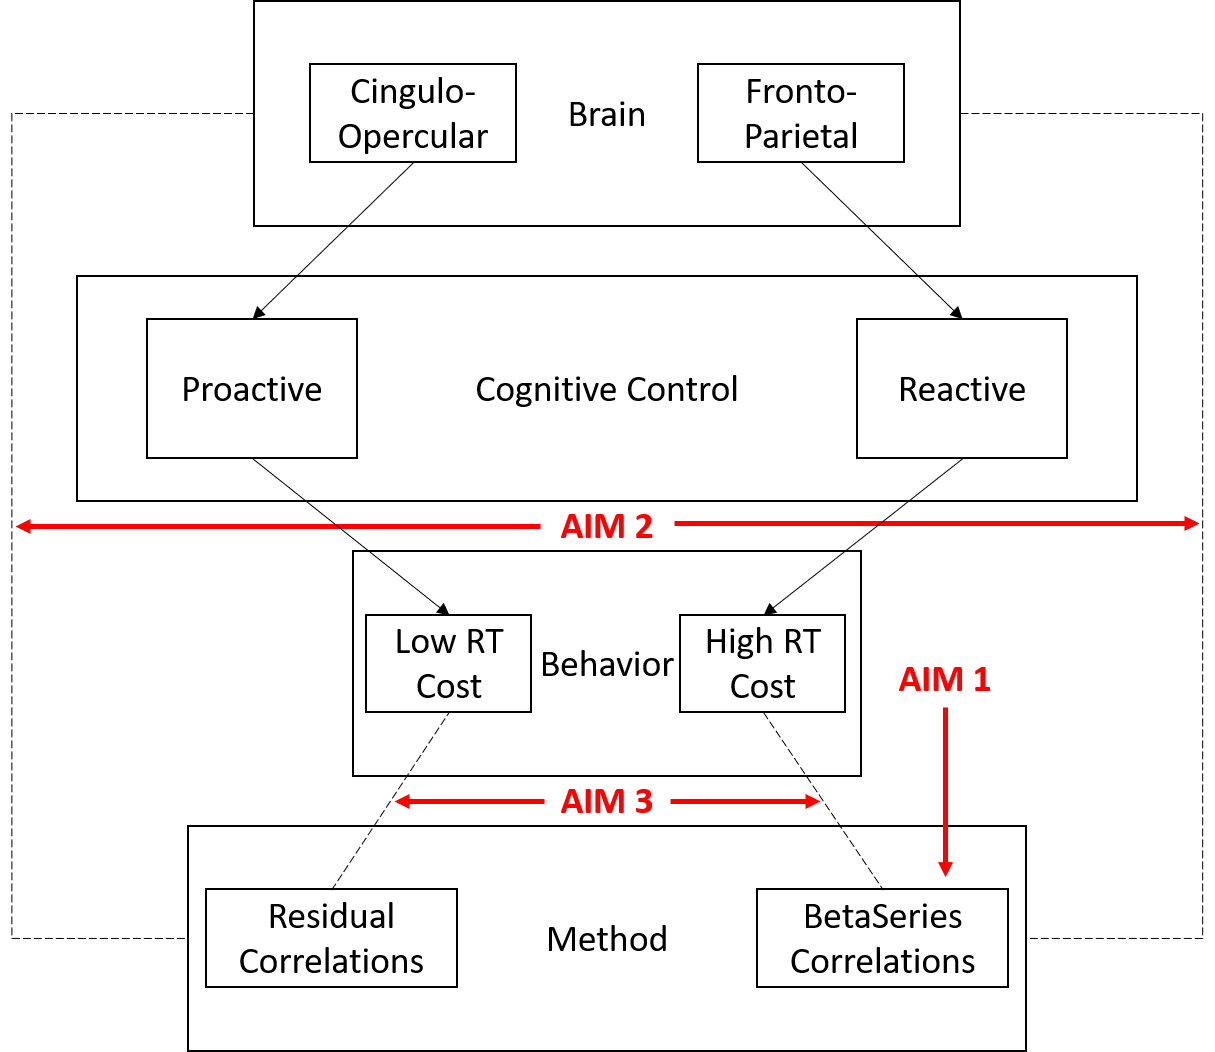
\includegraphics[width=1\linewidth]{all_aims}
	\caption{Outline of my three aims. Aim 1 seeks to produce and validate software developed with nipype to perform beta series correlations. Aim 2 will profile beta series correlations and residual correlations on the same task datasets to derive differences and similarities between the methods. Finally, Aim 3 connects the correlations derived from the two methods and compares them to behavioral measures of cognitive control (e.g. reaction time cost). Abbreviations: RT=reaction time}
	\label{fig:all_aims}
\end{figure}

\textbf{Specific Aim 1}: Create and validate a program to perform beta series correlations
\newline
\newline
\textit{Rationale}: A beta in this context refers to the free varying parameter in the general linear model (GLM) that "fits" the data.
\begin{equation}
	Y = X\beta + \epsilon 
	\label{eq:1}
\end{equation}
Equation \ref{eq:1} is the classic GLM where $Y$ represents the time-series we are attempting to explain.
The $\beta$ assumes any value that minimizes the squared error between the modeled data and the actual data. 
$\epsilon$ refers to the error that is not captured by the model.
\begin{equation} \label{eq:2}
Y = X_{Ti}\beta + \epsilon
\end{equation}
Equation \ref{eq:2} describes the least squares separate (LSS) implementation of a GLM, where the major difference is in the design term $X_{Ti}\beta$.
This notation represents that a particular ($Ti$) trial's $\beta$ is being estimated and not the average of all the trials.
Another detail not explicitly noted in the equation is that all other trials of the same type are treated as a single nuisance regressor.
The particular trial's $\beta$ will only account for the unique variance described by that trial.
If there are other trial types, each unique trial type will be its own nuisance regressor containing all trials of that type.
Thus we can account for the unique trial-to-trial variability of the betas.
\begin{algorithm}
	\caption{Beta Series Algorithm}\label{al:1}
	\begin{algorithmic}[1]
		\FOR{\texttt{Ti in Trials}}
    		\STATE \texttt{$Y = X_{Ti}\beta + \epsilon$}
		\ENDFOR
	\end{algorithmic}
\end{algorithm}
The algorithm to calculate each trial's $\beta$ estimate will be iteratively performed across trials and depending on the trial's condition (e.g. congruent vs. incongruent), the $\beta$ value will be placed in its corresponding list (Algorithm ~\ref{al:1}).
While programs exist to compute beta series correlations, there isn't one that utilizes least squares separate estimation, a modeling strategy that would help with deriving betas from fast event related designs with beta series correlations ~\citep{Mumford2012,Gottlich2015}. 
The proposed software seeks to fill that gap (Figure ~\ref{fig:all_aims}).
\newline
\newline
\textit{Hypothesis}:
The beta series software will capture brain response variability across trials to produce correlations that are different from resting state correlations.
\newline
\newline
\textit{Method}:
Under the Nipype framework, I will use python to model data on a trial-by-trial basis ~\citep{Smith2004,Gorgolewski2017}. 
Using a traditional GLM with a double gamma basis function, modeling will be completed by performing a GLM for each trial individually, with all other trials of the same type combined into a single term to form a regressor of non-interest ~\citep{Mumford2012}.
Additionally, trials from other trial types will each get their own regressor.

Validation of the beta series software will be shown progressively from simulations to real data.
Starting from simulations, two voxels will be simulated with a specified correlation of BOLD responses that I control.
I will vary the correlation between the two voxels and inject different amounts of noise to ascertain how well nibetaseries recaptures the correlation I set between the two voxels.
From these simulations I will be able to approximate power for subsequent analyses.
 
The next level of validation will proceed by comparing task data with resting state data.
The resting state data will be analytically treated the same as the task data, testing the assertion nibetaseries uses the BOLD response to capture correlations between brain regions.
Brain regions and networks will be defined with the Schaefer 400 atlas ~\citep{schaefer2017}.
The number of trials for a specific trial type will be divided into two sets and the difference of the correlation matrices between the two sets will determine the reliability of the correlation within task data.
The task correlation matrix will also be subtracted from the resting state correlation matrix to test whether BOLD responses from a task improves the reliability of beta series correlations.
Specifically, the comparison will be generated by: 1) subtracting one correlation matrix from another, 2) taking the absolute value of the differences, and 3) adding up the individual values.
I hypothesize the reliability within the task data will be greater than the reliability between task and rest.
The hypothesis will be tested with a paired-sample ttest, comparing the difference between the two sets of a single trial type for the task data and the difference between the task trial type set and the resting state set.
 
The final level of validation will be identical to the previous analysis, except the resting state data will have simulated task evoked responses inserted creating “pseudo-task” data.
The resting state data will be convolved with a hemodynamic response that represents the average response for each unique trial type for a participant.
For every occurance of a trial, the corresponding hemodynamic response will be fit to every voxel.
If engaging in a task only adds BOLD responses to the ongoing resting state activity, the correlation matrices from the “pseudo-task” data and the task data should be close to each other.
However, if there is variance in the BOLD response that is independent of the ongoing resting state activity, the correlation matrices from the “pseudo-task” data and the task data should be different.
This test may provide evidence that beta series correlations capture unique variance not explained by resting state fluctuations, validating the utility of beta series correlations to answer novel questions about brain activity during a task.
\newline
\newline
\textit{Alternative Methods}: If the beta series approach introduces bias into the correlation measures (e.g., all regions are strongly correlated with each other), the method to derive betas will be re-evaluated.
If there is not a suitable method to reduce/remove the bias, psycho-physiological interactions (PPI) may be used instead to derive relative trial activation, although there is no a priori reason to believe PPI will be less susceptible to bias.
In addition to taking absolute differences between correlation matrices, spatial correlations between matrices would indicate the similarity of the overall pattern of correlations.
To ensure the results are specific to a particular parcellation of the brain regions the Power atlas may be used to replicate the results.
\newline
\newline
\textbf{Specific Aim 2}: Characterize the relationship between beta series correlations (reactive) and residual correlations (proactive) during cognitive control tasks.
\newline
\newline
\textit{Rationale}: The dual mechanisms of control theory posits these networks should be differentially sensitive to the type of correlation method applied ~\citep{Dosenbach2007,Braver2006}.
However, work by Michael Cole suggests there will not be large differences between residual correlations and beta series correlations ~\citep{Cole2019}.
Despite the suggestion by Michael Cole's work, the differences between residual correlations and beta series correlations have not been explicitly tested.
This gap presenting an excellent opportunity to conceptually frame task data into stimulus evoked components and persistent residual components.
\newline
\newline
\textit{Hypothesis}:
I hypothesize the cingulo-opercular network will be modulated by proactive cognitive control and will be detectable with residual time series, but not beta series.
My complementary hypothesis states the frontal-parietal network will be modulated by reactive cognitive control and will be detectable with beta series, but not residual time series. 
\newline
\newline
\textit{Methods}:
Data from the openneuro dataset \href{https://openneuro.org/datasets/ds001751/versions/1.0.0}{ds001751} will be used to measure both beta series and residual correlations during a Flanker task.
The task has two block types, mostly incongruent (80 percent incongruent) and mostly congruent (20 percent incongruent).
The mostly incongruent block incites proactive cognitive control because the participant is likely to have to resolve a stimulus conflict for each trial.
On the other hand, the mostly congruent block encourages reactive control because the participant is not likely to see a conflicting stimulus.
All participants went through both congruent and incongruent blocks constituting a fully within subjects design.
The behavioral results indicate a successful manipulation of the congruency effect ~\citep{Aben2019}.
The participants had a much smaller congruency effect (measured with reaction timeseries) during the mostly incongruent block relative to the mostly congruent block.
For each participant, I will be able to measure both beta series correlations and residual correlations during mostly incongruent blocks and mostly congruent blocks. 
Using the Dosenbach ROIs, I will create correlation matrices for both beta series and residual time series ~\citep{Dosenbach2010}.
I will test the robustness of the results using the schafer atlas as an alternative atlas ~\citep{schaefer2017}.

To calculate residual correlations four steps will be completed.
First, the stimulus responses will be modeled and removed from the data.
To remove the stimulus responses, stimulus onsets from the task will be represented as impulses and convolved with a double gamma as the basis function for the GLM. 
Each stimulus event will entered into the GLM as its own regressor.
This ensures the trial-to-trial variance will be removed from the task data, and not just the mean response of a stimulus. 
The residual data from the GLM will represent BOLD responses not captured by direct responses to stimuli. 
Second, the data will be split into the mostly congruent block and mostly incongruent blocks.
The splitting allows me to analyze the state dependent correlations during the mostly congruent and mostly incongruent blocks separately.
Third, the data will be z-transformed to normalize the distributions and Pearson's R correlations will be extracted from ROIs that participate in the fronto-parietal network and the cingulo-opercular network.
Fourth, ROIs that belong to the same network will be correlated with each other and averaged giving an average within network correlation.

The beta series calculation will be done as described in aim 1.
The correlations will be performed similarly to the residual correlations, except instead of residuals, the beta maps will be normalized and ROI-ROI correlations will be performed for the incongruent trial type.
Average within network correlations for the cingulo-opercular and fronto-parietal networks across participants for both beta series and residual correlations in the mostly incongruent block and mostly congruent block serve as the primary outcome data.
I will look at change in within network correlations as a function of the network (fronto-parietal and cingulo-opercular) by block (mostly incongruent and mostly congruent) by method (residual and beta series correlations) using mixed effects modeling with a random intercept for participant.
I predict a significant network by block by method interaction.
From this interaction I expect the within network residual correlations from the cingulo-opercular network to increase during the mostly incongruent block relative to the mostly congruent block.
This prediction supports the proactive role of the cingulo-opercular network which is proposed to be online during the entirety of the mostly incongruent block.
I also expect the within network beta series correlations from the fronto-parietal network to increase during the mostly congruent block relative to the mostly incongruent block.
This prediction supports the reactive role of the fronto-parietal network which is only called upon during the incongruent trials within the mostly incongruent block.
\newline
\newline
\textit{Alternative Methods}:
Beta series correlations give correlations for each trial type (incongruent and congruent), but in the proposed methods I only anticipate the incongruent trials to have explanatory power.
However, it could be the relationship between congruent and incongruent trial types changes between the blocks suggesting subtracting the congruent correlation matrix from the incongruent correlation matrix would be more sensitive to the difference between blocks.
The mixed effects regression may also contain quality metrics of the data including average framewise displacement and global correlation to rule out noise driving the observed effect. 
If within network correlations from mixed effects regression do not adequately model the differences, I can use graph theoretical measures such as participation coefficient and efficiency.
\newline

%=============================================================================
\chapter{NiBetaSeries}
%=============================================================================

Beta series correlations appeared exciting when initially produced ~\citep{Rissman2004},
but have been relegated to post-hoc analyses being used as almost an afterthought in many
publications (add citations).
There was a brief resurgence when Benjamin Turner, Jeannette Mumford, and Hunar Abdulrahman... repurposed
beta series for classification of different trial types; however beta series correlations
remained under used.
Beta series correlations give a lens into how the brain's organization changes depending
on cognitive state, the theoretical implications would be fruitful for the field of neuroscience.
Then why aren't more researchers looking at beta series correlations?
Surveying the existing toolboxes available for calculating beta series correlations reveals a
potential answer.
A couple toolboxes that calculate beta series include BASCO, pybetaseries, and pyMVPA.
However, BASCO has limitations on the number of methods you can use to generate beta series,
pybetaseries is no longer being actively developed, and pyMVPA requires the user to know
a decent amount of python to make use of their functions.
With the limitations of the current toolboxes and the relative anonyminity of beta series,
it comes with little surprise that many researchers do not use this method and instead reach for
more familiar analyses using General Linear Models (GLMs) or resting state correlations applied
to task data (add citation).

To change this trend and make beta series more accessible, I've created a toolbox called NiBetaSeries.
NiBetaSeries leverages the latest trends in the python neuroimaging world and adds to the flourishing
ecosystem of tools that share a core organizational philosophy.
This tool calculates betaseries correlations for the user and passes the beta series images themselves
for the user to decide what analysis method they wish to pursue.

With the creation of this toolbox, I can test another reason for the dearth of published materials on
beta series correlations.
Namely, most researchers may not have found any results with beta series correlations.
In this chapter; I will explore under what experimental conditions NiBetaSeries is useful and offer
recommendations for when to use the toolbox.

\section{Simulations}
Simulation in fMRI has a rich literature, with mutliple strategies varying along the axis
of practicality and accuracy.
For testing tools/methods on many different experimental designs; simulating the bloch equations
is too computationally intensive and simpler simulations can generate realistic data.
To this author's knowledge, the first accessible tool to generate simulated fMRI data is NeuRoSim (add citation).
NeuRoSim allows the user to create expected responses to stimuli, motion noise, physiological noise,
timeseries drift, and autocorrelation of the timeseries (add citation).
More recently, the python module fmrisim was released mirroring the functionality of NeuRoSim, making this tool
the ideal choice to test NiBetaSeries; another python application.


\section{Real Data}

%=============================================================================
\chapter{Beta Series versus Residual Correlations}
%=============================================================================

\section{Residual Correlations}

Talk all about Micheal Cole...



%=============================================================================
\appendix
%=============================================================================

%=============================================================================
\chapter{Sample Appendix}

\section{Appendix One}
\blindtext

\section{Appendix Two}
\blindtext

%=============================================================================
\chapter{Another Appendix}

\section{Appendix Three}
\blindtext


%=============================================================================
% bibliography
%=============================================================================
\interlinepenalty=10000	% prevents bib items from splitting across pages
\bibliographystyle{uithesis}
\bibliography{thesis} 

\end{document}